% Options for packages loaded elsewhere
\PassOptionsToPackage{unicode}{hyperref}
\PassOptionsToPackage{hyphens}{url}
\PassOptionsToPackage{dvipsnames,svgnames,x11names}{xcolor}
%
\documentclass[
  letterpaper,
  DIV=11,
  numbers=noendperiod]{scrartcl}

\usepackage{amsmath,amssymb}
\usepackage{iftex}
\ifPDFTeX
  \usepackage[T1]{fontenc}
  \usepackage[utf8]{inputenc}
  \usepackage{textcomp} % provide euro and other symbols
\else % if luatex or xetex
  \usepackage{unicode-math}
  \defaultfontfeatures{Scale=MatchLowercase}
  \defaultfontfeatures[\rmfamily]{Ligatures=TeX,Scale=1}
\fi
\usepackage{lmodern}
\ifPDFTeX\else  
    % xetex/luatex font selection
\fi
% Use upquote if available, for straight quotes in verbatim environments
\IfFileExists{upquote.sty}{\usepackage{upquote}}{}
\IfFileExists{microtype.sty}{% use microtype if available
  \usepackage[]{microtype}
  \UseMicrotypeSet[protrusion]{basicmath} % disable protrusion for tt fonts
}{}
\makeatletter
\@ifundefined{KOMAClassName}{% if non-KOMA class
  \IfFileExists{parskip.sty}{%
    \usepackage{parskip}
  }{% else
    \setlength{\parindent}{0pt}
    \setlength{\parskip}{6pt plus 2pt minus 1pt}}
}{% if KOMA class
  \KOMAoptions{parskip=half}}
\makeatother
\usepackage{xcolor}
\setlength{\emergencystretch}{3em} % prevent overfull lines
\setcounter{secnumdepth}{-\maxdimen} % remove section numbering
% Make \paragraph and \subparagraph free-standing
\makeatletter
\ifx\paragraph\undefined\else
  \let\oldparagraph\paragraph
  \renewcommand{\paragraph}{
    \@ifstar
      \xxxParagraphStar
      \xxxParagraphNoStar
  }
  \newcommand{\xxxParagraphStar}[1]{\oldparagraph*{#1}\mbox{}}
  \newcommand{\xxxParagraphNoStar}[1]{\oldparagraph{#1}\mbox{}}
\fi
\ifx\subparagraph\undefined\else
  \let\oldsubparagraph\subparagraph
  \renewcommand{\subparagraph}{
    \@ifstar
      \xxxSubParagraphStar
      \xxxSubParagraphNoStar
  }
  \newcommand{\xxxSubParagraphStar}[1]{\oldsubparagraph*{#1}\mbox{}}
  \newcommand{\xxxSubParagraphNoStar}[1]{\oldsubparagraph{#1}\mbox{}}
\fi
\makeatother

\usepackage{color}
\usepackage{fancyvrb}
\newcommand{\VerbBar}{|}
\newcommand{\VERB}{\Verb[commandchars=\\\{\}]}
\DefineVerbatimEnvironment{Highlighting}{Verbatim}{commandchars=\\\{\}}
% Add ',fontsize=\small' for more characters per line
\usepackage{framed}
\definecolor{shadecolor}{RGB}{241,243,245}
\newenvironment{Shaded}{\begin{snugshade}}{\end{snugshade}}
\newcommand{\AlertTok}[1]{\textcolor[rgb]{0.68,0.00,0.00}{#1}}
\newcommand{\AnnotationTok}[1]{\textcolor[rgb]{0.37,0.37,0.37}{#1}}
\newcommand{\AttributeTok}[1]{\textcolor[rgb]{0.40,0.45,0.13}{#1}}
\newcommand{\BaseNTok}[1]{\textcolor[rgb]{0.68,0.00,0.00}{#1}}
\newcommand{\BuiltInTok}[1]{\textcolor[rgb]{0.00,0.23,0.31}{#1}}
\newcommand{\CharTok}[1]{\textcolor[rgb]{0.13,0.47,0.30}{#1}}
\newcommand{\CommentTok}[1]{\textcolor[rgb]{0.37,0.37,0.37}{#1}}
\newcommand{\CommentVarTok}[1]{\textcolor[rgb]{0.37,0.37,0.37}{\textit{#1}}}
\newcommand{\ConstantTok}[1]{\textcolor[rgb]{0.56,0.35,0.01}{#1}}
\newcommand{\ControlFlowTok}[1]{\textcolor[rgb]{0.00,0.23,0.31}{\textbf{#1}}}
\newcommand{\DataTypeTok}[1]{\textcolor[rgb]{0.68,0.00,0.00}{#1}}
\newcommand{\DecValTok}[1]{\textcolor[rgb]{0.68,0.00,0.00}{#1}}
\newcommand{\DocumentationTok}[1]{\textcolor[rgb]{0.37,0.37,0.37}{\textit{#1}}}
\newcommand{\ErrorTok}[1]{\textcolor[rgb]{0.68,0.00,0.00}{#1}}
\newcommand{\ExtensionTok}[1]{\textcolor[rgb]{0.00,0.23,0.31}{#1}}
\newcommand{\FloatTok}[1]{\textcolor[rgb]{0.68,0.00,0.00}{#1}}
\newcommand{\FunctionTok}[1]{\textcolor[rgb]{0.28,0.35,0.67}{#1}}
\newcommand{\ImportTok}[1]{\textcolor[rgb]{0.00,0.46,0.62}{#1}}
\newcommand{\InformationTok}[1]{\textcolor[rgb]{0.37,0.37,0.37}{#1}}
\newcommand{\KeywordTok}[1]{\textcolor[rgb]{0.00,0.23,0.31}{\textbf{#1}}}
\newcommand{\NormalTok}[1]{\textcolor[rgb]{0.00,0.23,0.31}{#1}}
\newcommand{\OperatorTok}[1]{\textcolor[rgb]{0.37,0.37,0.37}{#1}}
\newcommand{\OtherTok}[1]{\textcolor[rgb]{0.00,0.23,0.31}{#1}}
\newcommand{\PreprocessorTok}[1]{\textcolor[rgb]{0.68,0.00,0.00}{#1}}
\newcommand{\RegionMarkerTok}[1]{\textcolor[rgb]{0.00,0.23,0.31}{#1}}
\newcommand{\SpecialCharTok}[1]{\textcolor[rgb]{0.37,0.37,0.37}{#1}}
\newcommand{\SpecialStringTok}[1]{\textcolor[rgb]{0.13,0.47,0.30}{#1}}
\newcommand{\StringTok}[1]{\textcolor[rgb]{0.13,0.47,0.30}{#1}}
\newcommand{\VariableTok}[1]{\textcolor[rgb]{0.07,0.07,0.07}{#1}}
\newcommand{\VerbatimStringTok}[1]{\textcolor[rgb]{0.13,0.47,0.30}{#1}}
\newcommand{\WarningTok}[1]{\textcolor[rgb]{0.37,0.37,0.37}{\textit{#1}}}

\providecommand{\tightlist}{%
  \setlength{\itemsep}{0pt}\setlength{\parskip}{0pt}}\usepackage{longtable,booktabs,array}
\usepackage{calc} % for calculating minipage widths
% Correct order of tables after \paragraph or \subparagraph
\usepackage{etoolbox}
\makeatletter
\patchcmd\longtable{\par}{\if@noskipsec\mbox{}\fi\par}{}{}
\makeatother
% Allow footnotes in longtable head/foot
\IfFileExists{footnotehyper.sty}{\usepackage{footnotehyper}}{\usepackage{footnote}}
\makesavenoteenv{longtable}
\usepackage{graphicx}
\makeatletter
\newsavebox\pandoc@box
\newcommand*\pandocbounded[1]{% scales image to fit in text height/width
  \sbox\pandoc@box{#1}%
  \Gscale@div\@tempa{\textheight}{\dimexpr\ht\pandoc@box+\dp\pandoc@box\relax}%
  \Gscale@div\@tempb{\linewidth}{\wd\pandoc@box}%
  \ifdim\@tempb\p@<\@tempa\p@\let\@tempa\@tempb\fi% select the smaller of both
  \ifdim\@tempa\p@<\p@\scalebox{\@tempa}{\usebox\pandoc@box}%
  \else\usebox{\pandoc@box}%
  \fi%
}
% Set default figure placement to htbp
\def\fps@figure{htbp}
\makeatother

\usepackage{booktabs}
\usepackage{longtable}
\usepackage{array}
\usepackage{multirow}
\usepackage{wrapfig}
\usepackage{float}
\usepackage{colortbl}
\usepackage{pdflscape}
\usepackage{tabu}
\usepackage{threeparttable}
\usepackage{threeparttablex}
\usepackage[normalem]{ulem}
\usepackage{makecell}
\usepackage{xcolor}
\usepackage{longtable}
\KOMAoption{captions}{tableheading}
\makeatletter
\@ifpackageloaded{caption}{}{\usepackage{caption}}
\AtBeginDocument{%
\ifdefined\contentsname
  \renewcommand*\contentsname{Table of contents}
\else
  \newcommand\contentsname{Table of contents}
\fi
\ifdefined\listfigurename
  \renewcommand*\listfigurename{List of Figures}
\else
  \newcommand\listfigurename{List of Figures}
\fi
\ifdefined\listtablename
  \renewcommand*\listtablename{List of Tables}
\else
  \newcommand\listtablename{List of Tables}
\fi
\ifdefined\figurename
  \renewcommand*\figurename{Figure}
\else
  \newcommand\figurename{Figure}
\fi
\ifdefined\tablename
  \renewcommand*\tablename{Table}
\else
  \newcommand\tablename{Table}
\fi
}
\@ifpackageloaded{float}{}{\usepackage{float}}
\floatstyle{ruled}
\@ifundefined{c@chapter}{\newfloat{codelisting}{h}{lop}}{\newfloat{codelisting}{h}{lop}[chapter]}
\floatname{codelisting}{Listing}
\newcommand*\listoflistings{\listof{codelisting}{List of Listings}}
\makeatother
\makeatletter
\makeatother
\makeatletter
\@ifpackageloaded{caption}{}{\usepackage{caption}}
\@ifpackageloaded{subcaption}{}{\usepackage{subcaption}}
\makeatother
\makeatletter
\@ifpackageloaded{tcolorbox}{}{\usepackage[skins,breakable]{tcolorbox}}
\makeatother
\makeatletter
\@ifundefined{shadecolor}{\definecolor{shadecolor}{HTML}{FF0000}}{}
\makeatother
\makeatletter
\makeatother
\makeatletter
\ifdefined\Shaded\renewenvironment{Shaded}{\begin{tcolorbox}[breakable, borderline west={3pt}{0pt}{shadecolor}, enhanced, frame hidden, interior hidden, boxrule=0pt, sharp corners]}{\end{tcolorbox}}\fi
\makeatother
\makeatletter
\@ifpackageloaded{fontawesome5}{}{\usepackage{fontawesome5}}
\makeatother

\usepackage{bookmark}

\IfFileExists{xurl.sty}{\usepackage{xurl}}{} % add URL line breaks if available
\urlstyle{same} % disable monospaced font for URLs
\hypersetup{
  pdfauthor={Sebastián Egaña Santibáñez ; Nicolás Leiva Díaz },
  colorlinks=true,
  linkcolor={blue},
  filecolor={Maroon},
  citecolor={Blue},
  urlcolor={Blue},
  pdfcreator={LaTeX via pandoc}}


\title{
\includegraphics[width=5cm]{Imagen1.jpg}\\
Finanzas en R}
\usepackage{etoolbox}
\makeatletter
\providecommand{\subtitle}[1]{% add subtitle to \maketitle
  \apptocmd{\@title}{\par {\large #1 \par}}{}{}
}
\makeatother
\subtitle{Regresión lineal y aplicaciones}
\author{Sebastián Egaña Santibáñez
\href{mailto:segana@fen.uchile}{\faIcon{inbox}} \and Nicolás Leiva Díaz
\href{mailto:nleivad@fen.uchile.cl}{\faIcon{inbox}}}
\date{}

\begin{document}
\maketitle


\begin{center}\rule{0.5\linewidth}{0.5pt}\end{center}

\section{Enlaces del profesor}\label{enlaces-del-profesor}

\href{https://segana.netlify.app}{\faIcon{link}}
https://segana.netlify.app

\href{https://github.com/sebaegana}{\faIcon{github}}
https://github.com/sebaegana

\href{https://www.linkedin.com/in/sebastian-egana-santibanez/}{\faIcon{linkedin}}
https://www.linkedin.com/in/sebastian-egana-santibanez/

\begin{center}\rule{0.5\linewidth}{0.5pt}\end{center}

\section{Regresión Lineal}\label{regresiuxf3n-lineal}

En términos simples, una regresión lineal corresponde al intento
matemático y estadístico de analizar como un conjunto de datos se adapta
o no a un comportamiento lineal, ya sea esta relación directa o no.

Por ejemplo la oferta en donde el precio depende de la cantidad
demandada:

\begin{equation}
Precio = \alpha + \beta * Cantidad
\end{equation}

Se asumía que la relación podía ser de la siguiente manera:

\begin{equation}
Precio = 2 + 2 * Cantidad
\end{equation}

La regresión lineal, corresponde al intento de estimar los valores del
intercepto o constante y de la pendiente utilizando un metodo
matemático, en base a una muestra para extrapolar el comportamiento de
una población y con esto haciendo uso de principios estadísticos. Por
ejemplo, pretendemos saber si la muestra utilizada nos permite confirmar
el signo de la pendiente y el valor de la misma.

\section{Proyección de demanda}\label{proyecciuxf3n-de-demanda}

Se tiene un proyecto para una empresa de exportación, en donde se
pretende realizar una estimación del Tipo de cambio nominal (TCN de
ahora en adelante).

\begin{itemize}
\tightlist
\item
  Pregunta ¿por qué podría ser relevante el TCN para un proyecto como
  este? ¿Existe otro tipo de proyectos en dónde también podría ser
  relevante?
\end{itemize}

Para esto, el especialista econométrico plantea que el TCN posee una
relación con variables como el precio del cobre (Pcu) y el dolar index
(DXY).

\begin{itemize}
\tightlist
\item
  ¿Cuál es la razón de pensar en que existe una relación entre el TCN y
  el PCU? ¿Para el DXY?
\end{itemize}

Esto corresponde a una parte importante de la modelación; plantear la
relación teórica entre las variables.

Se plantea el siguiente modelo:

\begin{equation}
TCN = \alpha - \beta * Pcu
\end{equation}

Por otra parte, también podría ser:

\begin{equation}
TCN = \alpha + \beta * DXY
\end{equation}

¿Cuál debería ser la relación entre cada variable y el TCN?, esto
corresponde a un paso previo de la estimación econométrica.

\subsection{Estimación del modelo}\label{estimaciuxf3n-del-modelo}

Vemos los modelos por separado:

\begin{Shaded}
\begin{Highlighting}[]
\FunctionTok{library}\NormalTok{(tidyverse)}
\FunctionTok{library}\NormalTok{(readxl)}

\NormalTok{ejemplo }\OtherTok{\textless{}{-}} \FunctionTok{read\_excel}\NormalTok{(}\StringTok{"ejemplo.xlsx"}\NormalTok{)}

\NormalTok{data }\OtherTok{\textless{}{-}}\NormalTok{ ejemplo }\SpecialCharTok{\%\textgreater{}\%} 
  \FunctionTok{mutate}\NormalTok{(}\AttributeTok{year =} \FunctionTok{substring}\NormalTok{(fecha, }\DecValTok{1}\NormalTok{, }\DecValTok{4}\NormalTok{),}
         \AttributeTok{ln\_tcn =} \FunctionTok{log}\NormalTok{(TCN),}
         \AttributeTok{ln\_dxy =} \FunctionTok{log}\NormalTok{(}\StringTok{\textasciigrave{}}\AttributeTok{DXY Index}\StringTok{\textasciigrave{}}\NormalTok{),}
         \AttributeTok{ln\_pcu =} \FunctionTok{log}\NormalTok{(Pcu))}

\NormalTok{data\_subset }\OtherTok{\textless{}{-}}\NormalTok{ data }\SpecialCharTok{\%\textgreater{}\%} 
  \FunctionTok{filter}\NormalTok{(year }\SpecialCharTok{\textgreater{}=} \DecValTok{2014}\NormalTok{)}

\NormalTok{modelo\_01 }\OtherTok{\textless{}{-}} \FunctionTok{lm}\NormalTok{(TCN }\SpecialCharTok{\textasciitilde{}} \StringTok{\textasciigrave{}}\AttributeTok{DXY Index}\StringTok{\textasciigrave{}}\NormalTok{, }\AttributeTok{data =}\NormalTok{ data\_subset)}

\FunctionTok{summary}\NormalTok{(modelo\_01)}
\end{Highlighting}
\end{Shaded}

\begin{verbatim}

Call:
lm(formula = TCN ~ `DXY Index`, data = data_subset)

Residuals:
    Min      1Q  Median      3Q     Max 
-78.329 -24.316  -7.695  11.964 150.390 

Coefficients:
             Estimate Std. Error t value Pr(>|t|)    
(Intercept) -124.5077    92.0229  -1.353     0.18    
`DXY Index`    8.3562     0.9744   8.575  7.9e-13 ***
---
Signif. codes:  0 '***' 0.001 '**' 0.01 '*' 0.05 '.' 0.1 ' ' 1

Residual standard error: 47.88 on 77 degrees of freedom
  (1 observation deleted due to missingness)
Multiple R-squared:  0.4885,    Adjusted R-squared:  0.4819 
F-statistic: 73.54 on 1 and 77 DF,  p-value: 7.904e-13
\end{verbatim}

\begin{Shaded}
\begin{Highlighting}[]
\NormalTok{modelo\_02 }\OtherTok{\textless{}{-}} \FunctionTok{lm}\NormalTok{(TCN }\SpecialCharTok{\textasciitilde{}}\NormalTok{ Pcu, }\AttributeTok{data =}\NormalTok{ data\_subset)}

\FunctionTok{summary}\NormalTok{(modelo\_02)}
\end{Highlighting}
\end{Shaded}

\begin{verbatim}

Call:
lm(formula = TCN ~ Pcu, data = data_subset)

Residuals:
   Min     1Q Median     3Q    Max 
-70.99 -36.83 -11.43  23.39 142.63 

Coefficients:
            Estimate Std. Error t value Pr(>|t|)    
(Intercept) 975.5807    49.1646  19.843  < 2e-16 ***
Pcu          -1.1565     0.1807  -6.402  1.1e-08 ***
---
Signif. codes:  0 '***' 0.001 '**' 0.01 '*' 0.05 '.' 0.1 ' ' 1

Residual standard error: 54.08 on 77 degrees of freedom
  (1 observation deleted due to missingness)
Multiple R-squared:  0.3473,    Adjusted R-squared:  0.3389 
F-statistic: 40.98 on 1 and 77 DF,  p-value: 1.103e-08
\end{verbatim}

Observamos la relación en un gráfico de dispersión:

\begin{Shaded}
\begin{Highlighting}[]
\FunctionTok{plot}\NormalTok{(data\_subset}\SpecialCharTok{$}\NormalTok{Pcu, data\_subset}\SpecialCharTok{$}\NormalTok{TCN, }
     \AttributeTok{pch =} \DecValTok{16}\NormalTok{, }\AttributeTok{cex =} \FloatTok{1.3}\NormalTok{, }\AttributeTok{col =} \StringTok{"blue"}\NormalTok{, }
     \AttributeTok{main =} \StringTok{"Relación TCN y Pcu"}\NormalTok{, }
     \AttributeTok{xlab =} \StringTok{"Pcu"}\NormalTok{, }\AttributeTok{ylab =} \StringTok{"TCN"}\NormalTok{)}

\FunctionTok{abline}\NormalTok{(}\FunctionTok{lm}\NormalTok{(TCN }\SpecialCharTok{\textasciitilde{}}\NormalTok{ Pcu, }\AttributeTok{data =}\NormalTok{ data\_subset))}
\end{Highlighting}
\end{Shaded}

\pandocbounded{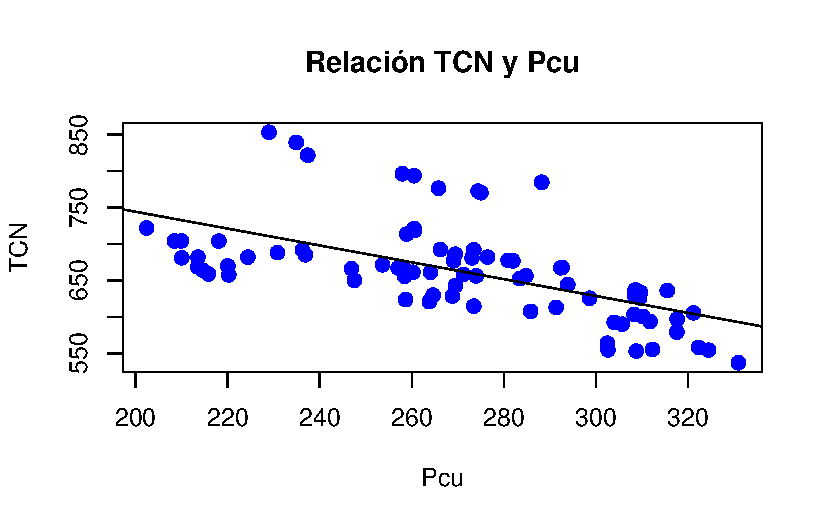
\includegraphics[keepaspectratio]{notebook_optimization_test_files/figure-pdf/unnamed-chunk-2-1.pdf}}

¿Cómo interpretaría usted estos valores?

¿Existe alguna particularidad en los valores de la estimación? Los
valores asociados a los parámetros estimados son particularmente grandes
(especialmente el valor de la constante).

Una solución a esto, muy utilizada en la práctica, es la utilización de
los logaritmos de las variables. Esto tiene dos ventajas:

\begin{enumerate}
\def\labelenumi{\arabic{enumi}.}
\tightlist
\item
  Soluciona problemas de escala.
\item
  Permite la interpretación en porcentajes.
\end{enumerate}

Con la regresión logaritmos:

\begin{Shaded}
\begin{Highlighting}[]
\NormalTok{modelo\_03 }\OtherTok{\textless{}{-}} \FunctionTok{lm}\NormalTok{(ln\_tcn }\SpecialCharTok{\textasciitilde{}}\NormalTok{ ln\_pcu, }\AttributeTok{data =}\NormalTok{ data\_subset)}

\FunctionTok{summary}\NormalTok{(modelo\_03)}
\end{Highlighting}
\end{Shaded}

\begin{verbatim}

Call:
lm(formula = ln_tcn ~ ln_pcu, data = data_subset)

Residuals:
     Min       1Q   Median       3Q      Max 
-0.11939 -0.05259 -0.01125  0.04046  0.20579 

Coefficients:
            Estimate Std. Error t value Pr(>|t|)    
(Intercept)  8.99887    0.39263  22.919  < 2e-16 ***
ln_pcu      -0.44835    0.07021  -6.386 1.18e-08 ***
---
Signif. codes:  0 '***' 0.001 '**' 0.01 '*' 0.05 '.' 0.1 ' ' 1

Residual standard error: 0.08006 on 77 degrees of freedom
  (1 observation deleted due to missingness)
Multiple R-squared:  0.3462,    Adjusted R-squared:  0.3377 
F-statistic: 40.78 on 1 and 77 DF,  p-value: 1.181e-08
\end{verbatim}

\begin{Shaded}
\begin{Highlighting}[]
\FunctionTok{plot}\NormalTok{(data\_subset}\SpecialCharTok{$}\NormalTok{ln\_pcu, data\_subset}\SpecialCharTok{$}\NormalTok{ln\_tcn, }
     \AttributeTok{pch =} \DecValTok{16}\NormalTok{, }\AttributeTok{cex =} \FloatTok{1.3}\NormalTok{, }\AttributeTok{col =} \StringTok{"blue"}\NormalTok{, }
     \AttributeTok{main =} \StringTok{"Relación TCN y Pcu"}\NormalTok{, }
     \AttributeTok{xlab =} \StringTok{"Ln Pcu"}\NormalTok{, }\AttributeTok{ylab =} \StringTok{"Ln TCN"}\NormalTok{)}

\FunctionTok{abline}\NormalTok{(}\FunctionTok{lm}\NormalTok{(ln\_tcn }\SpecialCharTok{\textasciitilde{}}\NormalTok{ ln\_pcu, }\AttributeTok{data =}\NormalTok{ data\_subset))}
\end{Highlighting}
\end{Shaded}

\pandocbounded{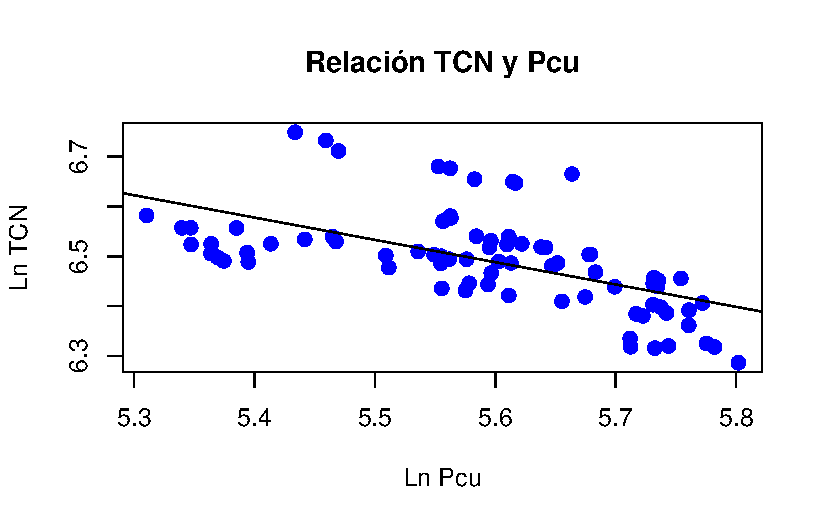
\includegraphics[keepaspectratio]{notebook_optimization_test_files/figure-pdf/unnamed-chunk-3-1.pdf}}

\subsection{¿Cómo analizar una
regresión?}\label{cuxf3mo-analizar-una-regresiuxf3n}

\begin{itemize}
\tightlist
\item
  Significancia individual
\end{itemize}

Por ejemplo para la constante, se evalua la siguiente hipótesis:

Hipótesis Nula o \(H_{0}\)

\begin{equation}
\beta_{1} = 0
\end{equation}

Hipótesis Alternativa o \(H_{1}\)

\begin{equation}
\beta_{1} \neq 0
\end{equation}

Se busca el poder rechazar la hipótesis nula, ¿pero por qué?

Este proceso se puede realizar de dos maneras (hay más):

\begin{itemize}
\tightlist
\item
  Estadístico calculado
\end{itemize}

Por ejemplo para el caso de la constante, este valor corresponde a 2,081
según la siguiente fórmula:

\begin{equation}
t_{calculado} = \frac{Coeficiente}{\text{error estándar del coeficiente}}
\end{equation}

lo que debe contrastarse con valores de tabla, según el siguiente
detalle:

\begin{equation}
t_{tabla} = t-student_{10\%, n - 1}
\end{equation}

Este valor de probabilidad se evalua generalmente al 10\%, al 5\% y al
1\%, y se le denomina valor significativo.

\begin{itemize}
\tightlist
\item
  P-Valor
\end{itemize}

Corresponde a la probabilidad acumulada por el valor t calculado,
considerando el espacio desde el estadístico hacia el final o inicio de
la distibución.

Se contrasta contra el valor de significancia. En caso de P-valor sea
menor que el nivel de significancia, ya sea (1\%, 5\% o 10\%), se
rechaza la hipótesis nula.

\begin{itemize}
\tightlist
\item
  Significancia global
\end{itemize}

Se aplica lo mismo, pero considerando el siguiente test:

Hipótesis Nula o \(H_{0}\)

\begin{equation}
\beta_{2} = \beta_{3}...\beta_{n} = 0
\end{equation}

Hipótesis Alternativa o \(H_{1}\)

\begin{equation}
\beta_{2} = \beta_{3}...\beta_{n} \neq 0
\end{equation}

No se considera la constante con una distribución F.

\begin{itemize}
\tightlist
\item
  Bondad del Ajuste
\end{itemize}

Se relaciona con el valor del R cuadrado y R cuadrado ajustado. Nos
habla del ajuste lineal del modelo. El segundo considera el ajuste por
el número de variables independientes.

Veamos esto en relación al último modelo calculado:

\begin{Shaded}
\begin{Highlighting}[]
\NormalTok{modelo\_03 }\OtherTok{\textless{}{-}} \FunctionTok{lm}\NormalTok{(ln\_tcn }\SpecialCharTok{\textasciitilde{}}\NormalTok{ ln\_pcu, }\AttributeTok{data =}\NormalTok{ data\_subset)}

\FunctionTok{summary}\NormalTok{(modelo\_03)}
\end{Highlighting}
\end{Shaded}

\begin{verbatim}

Call:
lm(formula = ln_tcn ~ ln_pcu, data = data_subset)

Residuals:
     Min       1Q   Median       3Q      Max 
-0.11939 -0.05259 -0.01125  0.04046  0.20579 

Coefficients:
            Estimate Std. Error t value Pr(>|t|)    
(Intercept)  8.99887    0.39263  22.919  < 2e-16 ***
ln_pcu      -0.44835    0.07021  -6.386 1.18e-08 ***
---
Signif. codes:  0 '***' 0.001 '**' 0.01 '*' 0.05 '.' 0.1 ' ' 1

Residual standard error: 0.08006 on 77 degrees of freedom
  (1 observation deleted due to missingness)
Multiple R-squared:  0.3462,    Adjusted R-squared:  0.3377 
F-statistic: 40.78 on 1 and 77 DF,  p-value: 1.181e-08
\end{verbatim}

\subsection{¿Cómo aplicamos esto?}\label{cuxf3mo-aplicamos-esto}

Teniendo las estimaciones del tipo de cambio, deberíamos poder generar
las estimaciones de las cantidades a vender. Conociendo el precio,
podríamos multiplicar todos los factores y obtenemos nuestro valor
inicial.

Por ejemplo:

\begin{equation}
Ventas_{year 1} = TCN_{year 1} * Cantidad_{year 1} = 720 * 1.000 = 720.000
\end{equation}

\begin{itemize}
\tightlist
\item
  ¿Ve algún problema en esto?
\end{itemize}

Desde este punto, solo queda poder aplicar un crecimiento a estas ventas
para los otros años a estimar.

Esto podemos explicarlo partiendo desde una pregunta:

\begin{itemize}
\item
  Tiene dos modelos de estimación de sus ventas: el primero, en base a
  un modelo econométrico y el segundo en base a una pregunta realizada a
  sus propios vendedores, sobre cuánto esperan vender ellos. ¿En cuál
  estimación o proyección confía más?
\item
  Por lo demás, existe un problema práctico sobre dichos modelos, si lo
  vemos en su especificación estimamos el siguiente modelo:
\end{itemize}

\begin{equation}
TCN = \alpha + \beta * Pcu
\end{equation}

¿Cuál es la temporalidad de la estimación? ¿Qué implica esto?

\section{Modelo CAPM}\label{modelo-capm}

Debemos ahora aplicar los contenidos vistos relacionados con regresión
simple. Un caso conocido en finanzas corresponde al modelo CAPM, que
relaciona los retornos de un activos o portafolio con los retornos del
mercado.

En base a esto, sabemos que la regresión simple posee la siguiente
especificación teórica:

\[ y = \alpha + \beta * x \]

n donde \(y\) corresponde a la variable dependiente, \(x\) corresponde a
la variable independiente, \(\alpha\) corresponde al intercepto y
\(\beta\) corresponde a la pendiente.

Dicho ejercicio corresponde al intento de estimar de manera empirica los
valores para una ecuación lineal; anteriormente los ejercicios que
utilizan ecuaciones de este tipo asumían los valores dados y no
ahondaban en el análisis estadístico que hay detrás de su estimación.

En base a esto CAPM en términos estimados corresponde a lo siguiente:

\[
r_{activo} = \hat{\alpha} + \hat{\beta} * r_{mercado}
\]

\begin{center}\rule{0.5\linewidth}{0.5pt}\end{center}

\section{Librerías a utilizar}\label{libreruxedas-a-utilizar}

Se especificas a continuación las libreríass que serán utilizados en
dicha sesión

\begin{Shaded}
\begin{Highlighting}[]
\FunctionTok{library}\NormalTok{(tidyquant)}
\FunctionTok{library}\NormalTok{(tidyverse)}
\FunctionTok{library}\NormalTok{(quantmod)}
\FunctionTok{library}\NormalTok{(timetk)}
\FunctionTok{library}\NormalTok{(broom)}
\FunctionTok{library}\NormalTok{(highcharter)}
\FunctionTok{library}\NormalTok{(ggpmisc)}
\FunctionTok{library}\NormalTok{(knitr)}
\FunctionTok{library}\NormalTok{(kableExtra)}
\end{Highlighting}
\end{Shaded}

\section{Acciones a utilizar}\label{acciones-a-utilizar}

Para este ejemplo, utilizáremos acciones del mercado de EE.UU.

\begin{Shaded}
\begin{Highlighting}[]
\CommentTok{\# Tickers a descargar}

\NormalTok{symbols }\OtherTok{\textless{}{-}} \FunctionTok{c}\NormalTok{(}\StringTok{"SPY"}\NormalTok{,}\StringTok{"EFA"}\NormalTok{, }\StringTok{"IJS"}\NormalTok{, }\StringTok{"EEM"}\NormalTok{,}\StringTok{"AGG"}\NormalTok{)}

\NormalTok{prices }\OtherTok{\textless{}{-}}
  \FunctionTok{getSymbols}\NormalTok{(symbols,}
             \AttributeTok{src =} \StringTok{\textquotesingle{}yahoo\textquotesingle{}}\NormalTok{,}
             \AttributeTok{from =} \StringTok{"2012{-}12{-}31"}\NormalTok{,}
             \AttributeTok{to =} \StringTok{"2021{-}12{-}31"}\NormalTok{,}
             \AttributeTok{auto.assign =} \ConstantTok{TRUE}\NormalTok{,}
             \AttributeTok{warnings =} \ConstantTok{FALSE}\NormalTok{) }\SpecialCharTok{\%\textgreater{}\%}
  \FunctionTok{map}\NormalTok{(}\SpecialCharTok{\textasciitilde{}}\FunctionTok{Ad}\NormalTok{(}\FunctionTok{get}\NormalTok{(.))) }\SpecialCharTok{\%\textgreater{}\%}
  \FunctionTok{reduce}\NormalTok{(merge) }\SpecialCharTok{\%\textgreater{}\%}
  \StringTok{\textasciigrave{}}\AttributeTok{colnames\textless{}{-}}\StringTok{\textasciigrave{}}\NormalTok{(symbols)}
\end{Highlighting}
\end{Shaded}

\subsection{Precios mensuales}\label{precios-mensuales}

Por lo general, el modelo CAPM se calcula utilizando ya sea precios
semanales o mensuales. En este caso utilizáremos precios mensuales.

\begin{Shaded}
\begin{Highlighting}[]
\CommentTok{\# Conversión a precios mensuales}

\NormalTok{prices\_monthly }\OtherTok{\textless{}{-}} \FunctionTok{to.monthly}\NormalTok{(prices,}
                             \AttributeTok{indexAt =} \StringTok{"lastof"}\NormalTok{,}
                             \AttributeTok{OHLC =} \ConstantTok{FALSE}\NormalTok{)}
\FunctionTok{head}\NormalTok{(prices\_monthly, }\DecValTok{3}\NormalTok{)}
\end{Highlighting}
\end{Shaded}

\begin{verbatim}
                SPY      EFA      IJS      EEM      AGG
2012-12-31 114.3474 39.29464 33.42036 33.69767 80.49226
2013-01-31 120.2008 40.75972 35.20887 33.59888 79.99228
2013-02-28 121.7345 40.23451 35.78303 32.83148 80.46491
\end{verbatim}

\subsection{Conversión a retornos}\label{conversiuxf3n-a-retornos}

Por lo general los retornos se calculan como la variación porcentual
entre dos fechas, en este caso mensuales. Una alternativa es calcularlo
utilizando variaciones en logaritmo lo que es muy utilizado por
profesionales de economía y finanzas.

Esto se puede cambiar variando el \texttt{method} entre
\texttt{"discrete",\ "log",\ "difference"}.

\begin{Shaded}
\begin{Highlighting}[]
\CommentTok{\# Cálculo del retorno usando logaritmos}

\NormalTok{asset\_returns\_xts }\OtherTok{\textless{}{-}}
  \FunctionTok{Return.calculate}\NormalTok{(prices\_monthly,}
                   \AttributeTok{method =} \StringTok{"log"}\NormalTok{) }\SpecialCharTok{\%\textgreater{}\%}
  \FunctionTok{na.omit}\NormalTok{()}

\FunctionTok{head}\NormalTok{(asset\_returns\_xts, }\DecValTok{3}\NormalTok{)}
\end{Highlighting}
\end{Shaded}

\begin{verbatim}
                  SPY         EFA        IJS          EEM           AGG
2013-01-31 0.04992309  0.03660632 0.05213273 -0.002935712 -0.0062309597
2013-02-28 0.01267844 -0.01296929 0.01617576 -0.023105116  0.0058911006
2013-03-31 0.03726805  0.01296929 0.04025823 -0.010235230  0.0009851312
\end{verbatim}

\subsection{Modificación y estructuración del data
frame}\label{modificaciuxf3n-y-estructuraciuxf3n-del-data-frame}

\begin{Shaded}
\begin{Highlighting}[]
\CommentTok{\# Generación de data frame desde archivo xts}

\NormalTok{asset\_returns\_dplyr\_byhand }\OtherTok{\textless{}{-}}
\NormalTok{  prices }\SpecialCharTok{\%\textgreater{}\%}
  \FunctionTok{to.monthly}\NormalTok{(}\AttributeTok{indexAt =} \StringTok{"lastof"}\NormalTok{, }\AttributeTok{OHLC =} \ConstantTok{FALSE}\NormalTok{) }\SpecialCharTok{\%\textgreater{}\%}
  \CommentTok{\# convert the index to a date}
  \FunctionTok{data.frame}\NormalTok{(}\AttributeTok{date =} \FunctionTok{index}\NormalTok{(.)) }\SpecialCharTok{\%\textgreater{}\%}
  \CommentTok{\# now remove the index because it got converted to row names}
  \FunctionTok{remove\_rownames}\NormalTok{() }\SpecialCharTok{\%\textgreater{}\%}
  \FunctionTok{gather}\NormalTok{(asset, prices, }\SpecialCharTok{{-}}\NormalTok{date) }\SpecialCharTok{\%\textgreater{}\%}
  \FunctionTok{group\_by}\NormalTok{(asset) }\SpecialCharTok{\%\textgreater{}\%}
  \FunctionTok{mutate}\NormalTok{(}\AttributeTok{returns =}\NormalTok{ (}\FunctionTok{log}\NormalTok{(prices) }\SpecialCharTok{{-}} \FunctionTok{log}\NormalTok{(}\FunctionTok{lag}\NormalTok{(prices)))) }\SpecialCharTok{\%\textgreater{}\%}
  \FunctionTok{select}\NormalTok{(}\SpecialCharTok{{-}}\NormalTok{prices) }\SpecialCharTok{\%\textgreater{}\%}
  \FunctionTok{spread}\NormalTok{(asset, returns) }\SpecialCharTok{\%\textgreater{}\%}
  \FunctionTok{select}\NormalTok{(date, }\FunctionTok{all\_of}\NormalTok{(symbols)) }\SpecialCharTok{\%\textgreater{}\%} 
  \FunctionTok{na.omit}\NormalTok{()}
\end{Highlighting}
\end{Shaded}

\section{Datos en formato long}\label{datos-en-formato-long}

\begin{Shaded}
\begin{Highlighting}[]
\CommentTok{\# Orientación del data frame en formato long}

\NormalTok{asset\_returns\_long }\OtherTok{\textless{}{-}}
\NormalTok{  asset\_returns\_dplyr\_byhand }\SpecialCharTok{\%\textgreater{}\%}
  \FunctionTok{gather}\NormalTok{(asset, returns, }\SpecialCharTok{{-}}\NormalTok{date) }\SpecialCharTok{\%\textgreater{}\%}
  \FunctionTok{group\_by}\NormalTok{(asset)}

\FunctionTok{head}\NormalTok{(asset\_returns\_long, }\DecValTok{3}\NormalTok{)}
\end{Highlighting}
\end{Shaded}

\begin{verbatim}
# A tibble: 3 x 3
# Groups:   asset [1]
  date       asset returns
  <date>     <chr>   <dbl>
1 2013-01-31 SPY    0.0499
2 2013-02-28 SPY    0.0127
3 2013-03-31 SPY    0.0373
\end{verbatim}

\subsection{Pesos de los activos dentro del
portafolio}\label{pesos-de-los-activos-dentro-del-portafolio}

En este caso, calcularémos el modelo CAPM para un portafolio de activos.
Para esto, debemos calcular el retorno ponderado del portafolio en base
a las distintas ponderaciones de cada activos en el portafolio.
Especificamos las ponderaciones:

\begin{Shaded}
\begin{Highlighting}[]
\CommentTok{\# Pesos para cálculo de portafolio}

\NormalTok{w }\OtherTok{\textless{}{-}} \FunctionTok{c}\NormalTok{(}\FloatTok{0.25}\NormalTok{,}
       \FloatTok{0.25}\NormalTok{,}
       \FloatTok{0.20}\NormalTok{,}
       \FloatTok{0.20}\NormalTok{,}
       \FloatTok{0.10}\NormalTok{)}
\end{Highlighting}
\end{Shaded}

\subsection{Cálculo del retorno del
portafolio}\label{cuxe1lculo-del-retorno-del-portafolio}

\begin{Shaded}
\begin{Highlighting}[]
\CommentTok{\# Cálculo del retorno ponderado del portafolio}

\NormalTok{portfolio\_returns\_tq\_rebalanced\_monthly }\OtherTok{\textless{}{-}}
\NormalTok{  asset\_returns\_long }\SpecialCharTok{\%\textgreater{}\%}
  \FunctionTok{tq\_portfolio}\NormalTok{(}\AttributeTok{assets\_col =}\NormalTok{ asset,}
               \AttributeTok{returns\_col =}\NormalTok{ returns,}
               \AttributeTok{weights =}\NormalTok{ w,}
               \AttributeTok{col\_rename =} \StringTok{"returns"}\NormalTok{,}
               \AttributeTok{rebalance\_on =} \StringTok{"months"}\NormalTok{)}
\end{Highlighting}
\end{Shaded}

\subsection{Histograma de los
retornos}\label{histograma-de-los-retornos}

\begin{Shaded}
\begin{Highlighting}[]
\CommentTok{\# Histograma de los retornos del portafolio}

\NormalTok{portfolio\_returns\_tq\_rebalanced\_monthly }\SpecialCharTok{\%\textgreater{}\%}
  \FunctionTok{ggplot}\NormalTok{(}\FunctionTok{aes}\NormalTok{(}\AttributeTok{x =}\NormalTok{ returns)) }\SpecialCharTok{+}
  \FunctionTok{geom\_histogram}\NormalTok{(}\AttributeTok{alpha =} \FloatTok{0.45}\NormalTok{, }\AttributeTok{binwidth =}\NormalTok{ .}\DecValTok{005}\NormalTok{) }\SpecialCharTok{+}
  \FunctionTok{ggtitle}\NormalTok{(}\StringTok{"Monthly Returns Since 2013"}\NormalTok{)}
\end{Highlighting}
\end{Shaded}

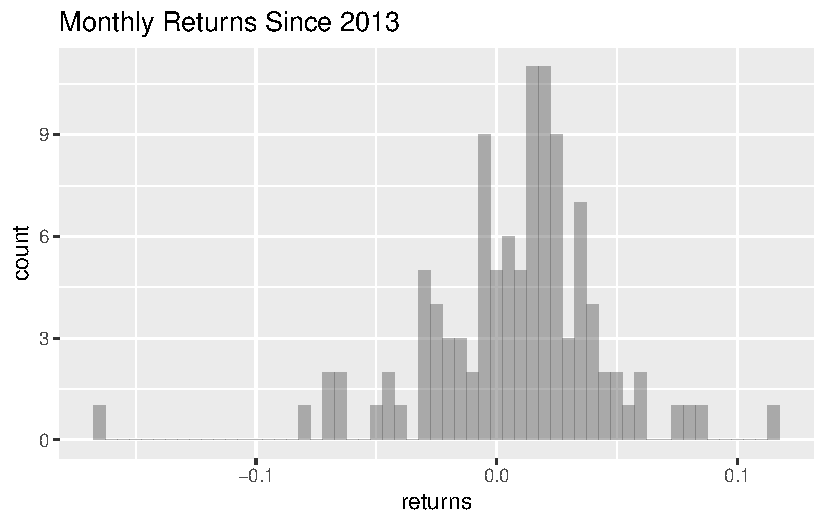
\includegraphics[width=0.5\linewidth,height=\textheight,keepaspectratio]{notebook_optimization_test_files/figure-pdf/unnamed-chunk-13-1.pdf}

\subsection{Histograma por activo}\label{histograma-por-activo}

\begin{Shaded}
\begin{Highlighting}[]
\CommentTok{\# Histograma de los retornos por activos}

\NormalTok{asset\_returns\_long }\SpecialCharTok{\%\textgreater{}\%}
  \FunctionTok{ggplot}\NormalTok{(}\FunctionTok{aes}\NormalTok{(}\AttributeTok{x =}\NormalTok{ returns, }\AttributeTok{fill =}\NormalTok{ asset)) }\SpecialCharTok{+}
  \FunctionTok{geom\_histogram}\NormalTok{(}\AttributeTok{alpha =} \FloatTok{0.45}\NormalTok{, }\AttributeTok{binwidth =}\NormalTok{ .}\DecValTok{01}\NormalTok{) }\SpecialCharTok{+} 
  \FunctionTok{facet\_wrap}\NormalTok{(}\SpecialCharTok{\textasciitilde{}}\NormalTok{asset) }\SpecialCharTok{+}
  \FunctionTok{ggtitle}\NormalTok{(}\StringTok{"Monthly Returns Since 2013"}\NormalTok{) }\SpecialCharTok{+}
  \FunctionTok{theme\_update}\NormalTok{(}\AttributeTok{plot.title =} \FunctionTok{element\_text}\NormalTok{(}\AttributeTok{hjust =} \FloatTok{0.5}\NormalTok{))}
\end{Highlighting}
\end{Shaded}

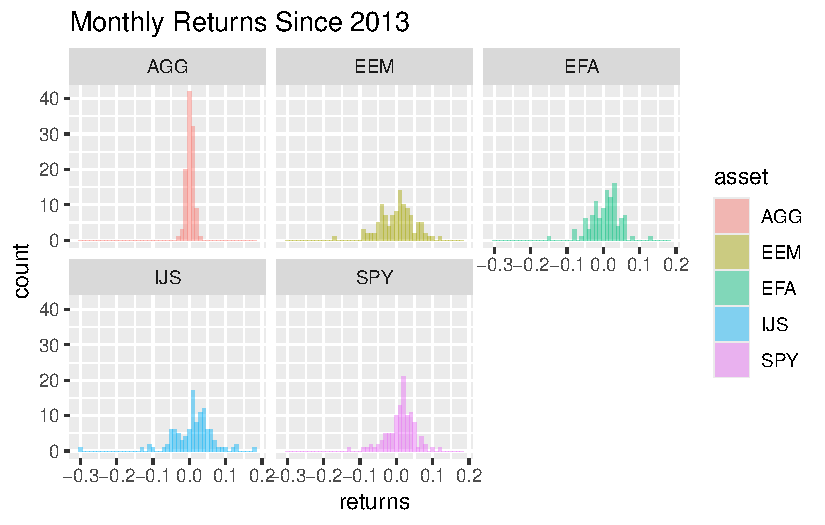
\includegraphics[width=0.5\linewidth,height=\textheight,keepaspectratio]{notebook_optimization_test_files/figure-pdf/unnamed-chunk-14-1.pdf}

\subsection{Histograma por activo
(variación)}\label{histograma-por-activo-variaciuxf3n}

\begin{Shaded}
\begin{Highlighting}[]
\CommentTok{\# Histograma de los retornos por activos}

\NormalTok{asset\_returns\_long }\SpecialCharTok{\%\textgreater{}\%}
  \FunctionTok{ggplot}\NormalTok{(}\FunctionTok{aes}\NormalTok{(}\AttributeTok{x =}\NormalTok{ returns)) }\SpecialCharTok{+}
  \FunctionTok{geom\_density}\NormalTok{(}\FunctionTok{aes}\NormalTok{(}\AttributeTok{color =}\NormalTok{ asset), }\AttributeTok{alpha =} \DecValTok{1}\NormalTok{) }\SpecialCharTok{+}
  \FunctionTok{geom\_histogram}\NormalTok{(}\FunctionTok{aes}\NormalTok{(}\AttributeTok{fill =}\NormalTok{ asset), }\AttributeTok{alpha =} \FloatTok{0.45}\NormalTok{, }\AttributeTok{binwidth =}\NormalTok{ .}\DecValTok{01}\NormalTok{) }\SpecialCharTok{+}
  \FunctionTok{guides}\NormalTok{(}\AttributeTok{fill =} \ConstantTok{FALSE}\NormalTok{) }\SpecialCharTok{+}
  \FunctionTok{facet\_wrap}\NormalTok{(}\SpecialCharTok{\textasciitilde{}}\NormalTok{asset) }\SpecialCharTok{+}
  \FunctionTok{ggtitle}\NormalTok{(}\StringTok{"Monthly Returns Since 2013"}\NormalTok{) }\SpecialCharTok{+}
  \FunctionTok{xlab}\NormalTok{(}\StringTok{"monthly returns"}\NormalTok{) }\SpecialCharTok{+}
  \FunctionTok{ylab}\NormalTok{(}\StringTok{"distribution"}\NormalTok{) }\SpecialCharTok{+}
  \FunctionTok{theme\_update}\NormalTok{(}\AttributeTok{plot.title =} \FunctionTok{element\_text}\NormalTok{(}\AttributeTok{hjust =} \FloatTok{0.5}\NormalTok{)) }\SpecialCharTok{+}
  \FunctionTok{guides}\NormalTok{(}\AttributeTok{scale =} \StringTok{"none"}\NormalTok{)}
\end{Highlighting}
\end{Shaded}

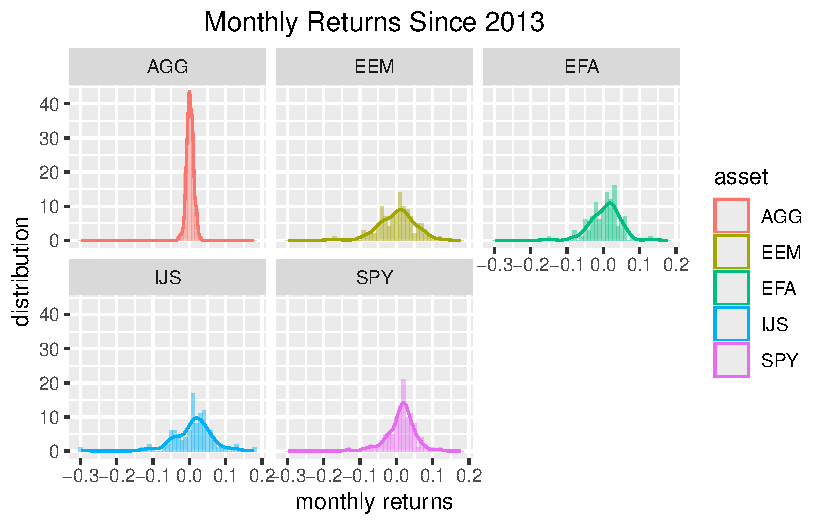
\includegraphics[width=0.4\linewidth,height=\textheight,keepaspectratio]{notebook_optimization_test_files/figure-pdf/unnamed-chunk-15-1.pdf}

\subsection{Gráfico de densidad}\label{gruxe1fico-de-densidad}

\begin{Shaded}
\begin{Highlighting}[]
\CommentTok{\# Densidad}

\NormalTok{portfolio\_density\_plot }\OtherTok{\textless{}{-}}
\NormalTok{  asset\_returns\_long }\SpecialCharTok{\%\textgreater{}\%}
  \FunctionTok{ggplot}\NormalTok{(}\FunctionTok{aes}\NormalTok{(}\AttributeTok{x =}\NormalTok{ returns)) }\SpecialCharTok{+}
  \FunctionTok{stat\_density}\NormalTok{(}\AttributeTok{geom =} \StringTok{"line"}\NormalTok{,}
               \AttributeTok{alpha =} \DecValTok{1}\NormalTok{,}
               \AttributeTok{colour =} \StringTok{"cornflowerblue"}\NormalTok{)}

\NormalTok{portfolio\_density\_plot}
\end{Highlighting}
\end{Shaded}

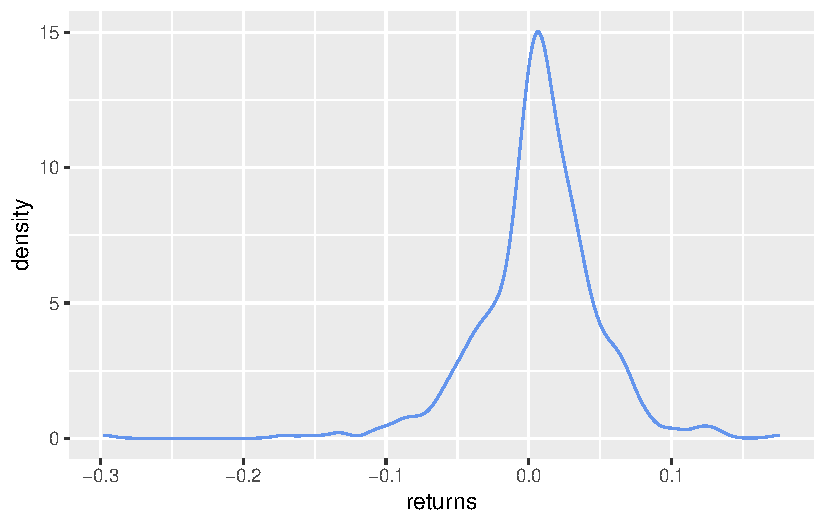
\includegraphics[width=0.4\linewidth,height=\textheight,keepaspectratio]{notebook_optimization_test_files/figure-pdf/unnamed-chunk-16-1.pdf}

\subsection{Grafico de densidad con área
sombreada}\label{grafico-de-densidad-con-uxe1rea-sombreada}

\begin{Shaded}
\begin{Highlighting}[]
\NormalTok{shaded\_area\_data }\OtherTok{\textless{}{-}}
  \FunctionTok{ggplot\_build}\NormalTok{(portfolio\_density\_plot)}\SpecialCharTok{$}\NormalTok{data[[}\DecValTok{1}\NormalTok{]] }\SpecialCharTok{\%\textgreater{}\%}
  \FunctionTok{filter}\NormalTok{(x }\SpecialCharTok{\textless{}} \FunctionTok{mean}\NormalTok{(asset\_returns\_long}\SpecialCharTok{$}\NormalTok{returns))}

\NormalTok{portfolio\_density\_plot\_shaded }\OtherTok{\textless{}{-}}
\NormalTok{  portfolio\_density\_plot }\SpecialCharTok{+}
  \FunctionTok{geom\_area}\NormalTok{(}\AttributeTok{data =}\NormalTok{ shaded\_area\_data,}
            \FunctionTok{aes}\NormalTok{(}\AttributeTok{x =}\NormalTok{ x, }\AttributeTok{y =}\NormalTok{ y),}
            \AttributeTok{fill=}\StringTok{"pink"}\NormalTok{,}
            \AttributeTok{alpha =} \FloatTok{0.5}\NormalTok{)}

\NormalTok{portfolio\_density\_plot\_shaded}
\end{Highlighting}
\end{Shaded}

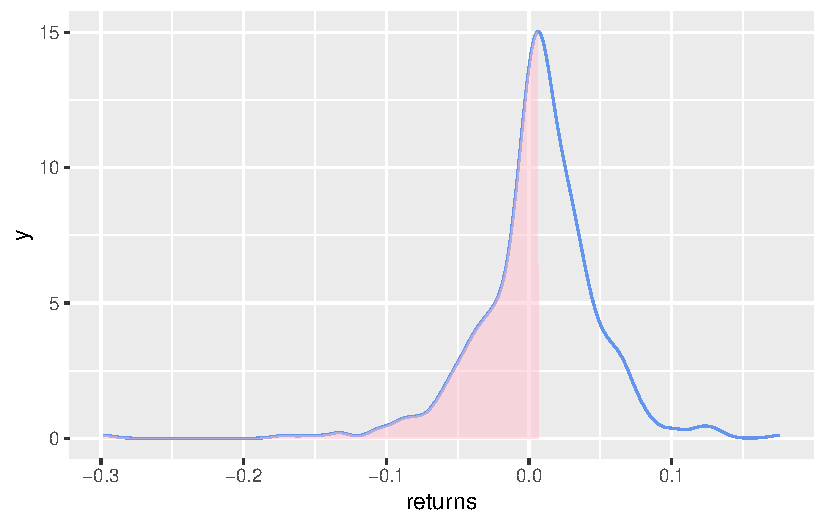
\includegraphics[width=0.4\linewidth,height=\textheight,keepaspectratio]{notebook_optimization_test_files/figure-pdf/unnamed-chunk-17-1.pdf}

\section{Retorno de Mercado}\label{retorno-de-mercado}

El retorno del mercado será aproximado desde el retorno del SPY

\begin{Shaded}
\begin{Highlighting}[]
\DocumentationTok{\#\# CAPM}

\NormalTok{market\_returns\_xts }\OtherTok{\textless{}{-}}
  \FunctionTok{getSymbols}\NormalTok{(}\StringTok{"SPY"}\NormalTok{,}
             \AttributeTok{src =} \StringTok{\textquotesingle{}yahoo\textquotesingle{}}\NormalTok{,}
             \AttributeTok{from =} \StringTok{"2012{-}12{-}31"}\NormalTok{,}
             \AttributeTok{to =} \StringTok{"2021{-}12{-}31"}\NormalTok{,}
             \AttributeTok{auto.assign =} \ConstantTok{TRUE}\NormalTok{,}
             \AttributeTok{warnings =} \ConstantTok{FALSE}\NormalTok{) }\SpecialCharTok{\%\textgreater{}\%}
  \FunctionTok{map}\NormalTok{(}\SpecialCharTok{\textasciitilde{}}\FunctionTok{Ad}\NormalTok{(}\FunctionTok{get}\NormalTok{(.))) }\SpecialCharTok{\%\textgreater{}\%}
  \FunctionTok{reduce}\NormalTok{(merge) }\SpecialCharTok{\%\textgreater{}\%}
  \StringTok{\textasciigrave{}}\AttributeTok{colnames\textless{}{-}}\StringTok{\textasciigrave{}}\NormalTok{(}\StringTok{"SPY"}\NormalTok{) }\SpecialCharTok{\%\textgreater{}\%}
  \FunctionTok{to.monthly}\NormalTok{(}\AttributeTok{indexAt =} \StringTok{"lastof"}\NormalTok{,}
             \AttributeTok{OHLC =} \ConstantTok{FALSE}\NormalTok{) }\SpecialCharTok{\%\textgreater{}\%}
  \FunctionTok{Return.calculate}\NormalTok{(.,}
                   \AttributeTok{method =} \StringTok{"log"}\NormalTok{) }\SpecialCharTok{\%\textgreater{}\%}
\NormalTok{  na.omit}

\NormalTok{market\_returns\_tidy }\OtherTok{\textless{}{-}}
\NormalTok{  market\_returns\_xts }\SpecialCharTok{\%\textgreater{}\%}
  \FunctionTok{tk\_tbl}\NormalTok{(}\AttributeTok{preserve\_index =} \ConstantTok{TRUE}\NormalTok{,}
         \AttributeTok{rename\_index =} \StringTok{"date"}\NormalTok{) }\SpecialCharTok{\%\textgreater{}\%}
  \FunctionTok{na.omit}\NormalTok{() }\SpecialCharTok{\%\textgreater{}\%}
  \FunctionTok{select}\NormalTok{(date, }\AttributeTok{returns =}\NormalTok{ SPY)}
\end{Highlighting}
\end{Shaded}

\subsection{Retorno de Mercado}\label{retorno-de-mercado-1}

\begin{Shaded}
\begin{Highlighting}[]
\NormalTok{portfolio\_returns\_xts\_rebalanced\_monthly }\OtherTok{\textless{}{-}}
  \FunctionTok{Return.portfolio}\NormalTok{(asset\_returns\_xts,}
                   \AttributeTok{weights =}\NormalTok{ w,}
                   \AttributeTok{rebalance\_on =} \StringTok{"months"}\NormalTok{) }\SpecialCharTok{\%\textgreater{}\%}
  \StringTok{\textasciigrave{}}\AttributeTok{colnames\textless{}{-}}\StringTok{\textasciigrave{}}\NormalTok{(}\StringTok{"returns"}\NormalTok{)}

\FunctionTok{head}\NormalTok{(portfolio\_returns\_xts\_rebalanced\_monthly, }\DecValTok{3}\NormalTok{)}
\end{Highlighting}
\end{Shaded}

\begin{verbatim}
                 returns
2013-01-31  0.0308486600
2013-02-28 -0.0008694719
2013-03-31  0.0186624462
\end{verbatim}

\subsection{\texorpdfstring{Calculo de los
\(\beta\)}{Calculo de los \textbackslash beta}}\label{calculo-de-los-beta}

Desarrollamos el modelo especificado al principio pero considerando cada
activo que compone al portafolio

\begin{Shaded}
\begin{Highlighting}[]
\NormalTok{beta\_assets }\OtherTok{\textless{}{-}}
\NormalTok{  asset\_returns\_long }\SpecialCharTok{\%\textgreater{}\%}
  \FunctionTok{nest}\NormalTok{(}\SpecialCharTok{{-}}\NormalTok{asset) }\SpecialCharTok{\%\textgreater{}\%}
  \FunctionTok{mutate}\NormalTok{(}\AttributeTok{model =}
           \FunctionTok{map}\NormalTok{(data, }\SpecialCharTok{\textasciitilde{}}
                 \FunctionTok{lm}\NormalTok{(returns }\SpecialCharTok{\textasciitilde{}}\NormalTok{ market\_returns\_tidy}\SpecialCharTok{$}\NormalTok{returns,}
                    \AttributeTok{data =}\NormalTok{ .))) }\SpecialCharTok{\%\textgreater{}\%}
  \FunctionTok{mutate}\NormalTok{(}\AttributeTok{model =} \FunctionTok{map}\NormalTok{(model, tidy)) }\SpecialCharTok{\%\textgreater{}\%}
  \FunctionTok{unnest}\NormalTok{(model) }\SpecialCharTok{\%\textgreater{}\%}
  \FunctionTok{mutate\_if}\NormalTok{(is.numeric, }\FunctionTok{list}\NormalTok{(}\SpecialCharTok{\textasciitilde{}} \FunctionTok{round}\NormalTok{(., }\DecValTok{4}\NormalTok{)))}


\NormalTok{beta\_assets\_show }\OtherTok{\textless{}{-}}\NormalTok{ beta\_assets }\SpecialCharTok{\%\textgreater{}\%} 
  \FunctionTok{select}\NormalTok{(}\SpecialCharTok{{-}}\NormalTok{data)}
\end{Highlighting}
\end{Shaded}

\begin{Shaded}
\begin{Highlighting}[]
\NormalTok{beta\_assets\_show}
\end{Highlighting}
\end{Shaded}

\begin{verbatim}
# A tibble: 10 x 6
# Groups:   asset [5]
   asset term                        estimate std.error    statistic p.value
   <chr> <chr>                          <dbl>     <dbl>        <dbl>   <dbl>
 1 SPY   (Intercept)                   0         0           -0.0013  0.999 
 2 SPY   market_returns_tidy$returns   1         0      1357133.      0     
 3 EFA   (Intercept)                  -0.0057    0.0021      -2.77    0.0066
 4 EFA   market_returns_tidy$returns   0.879     0.0513      17.1     0     
 5 IJS   (Intercept)                  -0.006     0.0033      -1.81    0.0735
 6 IJS   market_returns_tidy$returns   1.25      0.0816      15.4     0     
 7 EEM   (Intercept)                  -0.0081    0.0035      -2.33    0.0218
 8 EEM   market_returns_tidy$returns   0.844     0.0857       9.85    0     
 9 AGG   (Intercept)                   0.0022    0.0009       2.40    0.0183
10 AGG   market_returns_tidy$returns  -0.0009    0.0232      -0.0408  0.968 
\end{verbatim}

\subsection{Tabla con los
coeficientes}\label{tabla-con-los-coeficientes}

\begin{Shaded}
\begin{Highlighting}[]
\NormalTok{knitr}\SpecialCharTok{::}\FunctionTok{kable}\NormalTok{(}
\NormalTok{  beta\_assets\_show,}
  \AttributeTok{format =} \StringTok{"latex"}\NormalTok{,          }\CommentTok{\# or omit this if rendering to HTML}
  \AttributeTok{booktabs =} \ConstantTok{TRUE}\NormalTok{,}
  \AttributeTok{digits =} \DecValTok{2}
\NormalTok{)}
\end{Highlighting}
\end{Shaded}

\begin{tabular}{llrrrr}
\toprule
asset & term & estimate & std.error & statistic & p.value\\
\midrule
SPY & (Intercept) & 0.00 & 0.00 & 0.00 & 1.00\\
SPY & market\_returns\_tidy\$returns & 1.00 & 0.00 & 1357132.52 & 0.00\\
EFA & (Intercept) & -0.01 & 0.00 & -2.77 & 0.01\\
EFA & market\_returns\_tidy\$returns & 0.88 & 0.05 & 17.14 & 0.00\\
IJS & (Intercept) & -0.01 & 0.00 & -1.81 & 0.07\\
\addlinespace
IJS & market\_returns\_tidy\$returns & 1.25 & 0.08 & 15.37 & 0.00\\
EEM & (Intercept) & -0.01 & 0.00 & -2.33 & 0.02\\
EEM & market\_returns\_tidy\$returns & 0.84 & 0.09 & 9.85 & 0.00\\
AGG & (Intercept) & 0.00 & 0.00 & 2.40 & 0.02\\
AGG & market\_returns\_tidy\$returns & 0.00 & 0.02 & -0.04 & 0.97\\
\bottomrule
\end{tabular}

\section{Análisis}\label{anuxe1lisis}

Debemos realizar el análisis en base a los valores obtenidos para los
coeficientes. Cabe mencionar, que tenemos un mayor interés en encontrar
significancia en el parámetro relacionado con la pendiente y no en el
relacionado con el intercepto.

Por otra parte, ¿qué significa que el parámetro sea mayor o menor que 1?

\subsection{Análisis gráfico}\label{anuxe1lisis-gruxe1fico}

Podemos generar una regresión considerando que corresponde a la línea
que atraviesa entre los puntos de ambas variables. Para esto generamos
un gráfico de puntos entre X e Y, considerando la relación entre los
retornos del portafolio y los retornos del mercado.

\begin{Shaded}
\begin{Highlighting}[]
\NormalTok{portfolio\_returns\_tq\_rebalanced\_monthly }\SpecialCharTok{\%\textgreater{}\%}
  \FunctionTok{mutate}\NormalTok{(}\AttributeTok{market\_returns =}
\NormalTok{           market\_returns\_tidy}\SpecialCharTok{$}\NormalTok{returns) }\SpecialCharTok{\%\textgreater{}\%}
  \FunctionTok{ggplot}\NormalTok{(}\FunctionTok{aes}\NormalTok{(}\AttributeTok{x =}\NormalTok{ market\_returns,}
             \AttributeTok{y =}\NormalTok{ returns)) }\SpecialCharTok{+}
  \FunctionTok{geom\_point}\NormalTok{(}\AttributeTok{color =} \StringTok{"cornflowerblue"}\NormalTok{) }\SpecialCharTok{+}
  \FunctionTok{ylab}\NormalTok{(}\StringTok{"portfolio returns"}\NormalTok{) }\SpecialCharTok{+}
  \FunctionTok{xlab}\NormalTok{(}\StringTok{"market returns"}\NormalTok{)}
\end{Highlighting}
\end{Shaded}

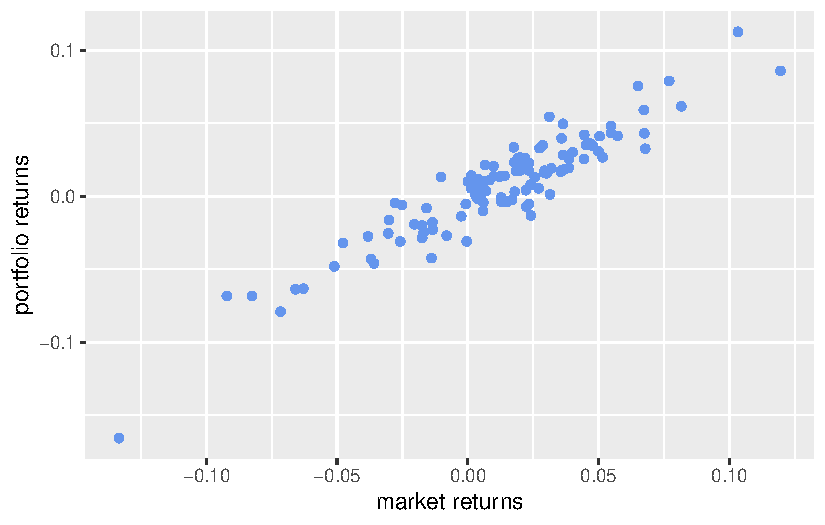
\includegraphics[width=0.4\linewidth,height=\textheight,keepaspectratio]{notebook_optimization_test_files/figure-pdf/unnamed-chunk-23-1.pdf}

\subsection{Línea de regresión}\label{luxednea-de-regresiuxf3n}

Utilizando el gráfico anterior, generamos la línea de regresión:

\begin{Shaded}
\begin{Highlighting}[]
\NormalTok{portfolio\_returns\_tq\_rebalanced\_monthly }\SpecialCharTok{\%\textgreater{}\%}
  \FunctionTok{mutate}\NormalTok{(}\AttributeTok{market\_returns =}
\NormalTok{           market\_returns\_tidy}\SpecialCharTok{$}\NormalTok{returns) }\SpecialCharTok{\%\textgreater{}\%}
  \FunctionTok{ggplot}\NormalTok{(}\FunctionTok{aes}\NormalTok{(}\AttributeTok{x =}\NormalTok{ market\_returns,}
             \AttributeTok{y =}\NormalTok{ returns)) }\SpecialCharTok{+}
  \FunctionTok{geom\_point}\NormalTok{(}\AttributeTok{color =} \StringTok{"cornflowerblue"}\NormalTok{) }\SpecialCharTok{+}
  \FunctionTok{geom\_smooth}\NormalTok{(}\AttributeTok{method =} \StringTok{"lm"}\NormalTok{,}
              \AttributeTok{se =} \ConstantTok{FALSE}\NormalTok{,}
              \AttributeTok{color =} \StringTok{"green"}\NormalTok{) }\SpecialCharTok{+}
  \FunctionTok{ylab}\NormalTok{(}\StringTok{"portfolio returns"}\NormalTok{) }\SpecialCharTok{+}
  \FunctionTok{xlab}\NormalTok{(}\StringTok{"market returns"}\NormalTok{)   }
\end{Highlighting}
\end{Shaded}

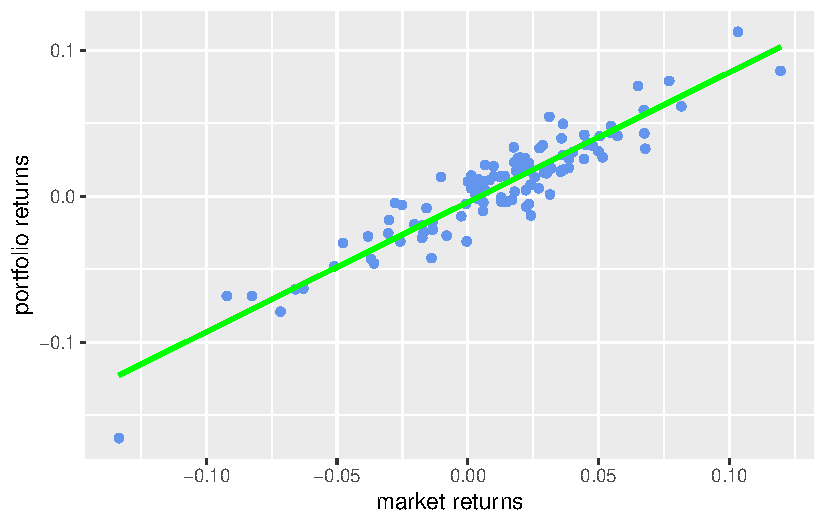
\includegraphics[width=0.4\linewidth,height=\textheight,keepaspectratio]{notebook_optimization_test_files/figure-pdf/unnamed-chunk-24-1.pdf}

\subsection{Gráfico con los parametros
calculados}\label{gruxe1fico-con-los-parametros-calculados}

Podemos también agregar al gráfico la éxpresión de la regresión
calculada:

\begin{Shaded}
\begin{Highlighting}[]
\NormalTok{data }\OtherTok{\textless{}{-}}\NormalTok{ portfolio\_returns\_tq\_rebalanced\_monthly }\SpecialCharTok{\%\textgreater{}\%}
  \FunctionTok{mutate}\NormalTok{(}\AttributeTok{market\_returns =}
\NormalTok{           market\_returns\_tidy}\SpecialCharTok{$}\NormalTok{returns) }

\NormalTok{my.formula }\OtherTok{\textless{}{-}}\NormalTok{ y }\SpecialCharTok{\textasciitilde{}}\NormalTok{ x}

\NormalTok{p }\OtherTok{\textless{}{-}} \FunctionTok{ggplot}\NormalTok{(}\AttributeTok{data =}\NormalTok{ data, }\FunctionTok{aes}\NormalTok{(}\AttributeTok{x =}\NormalTok{ market\_returns,}
                           \AttributeTok{y =}\NormalTok{ returns)) }\SpecialCharTok{+}
  \FunctionTok{geom\_smooth}\NormalTok{(}\AttributeTok{method =} \StringTok{"lm"}\NormalTok{, }\AttributeTok{se=}\ConstantTok{FALSE}\NormalTok{, }\AttributeTok{color=}\StringTok{"green"}\NormalTok{, }\AttributeTok{formula =}\NormalTok{ my.formula) }\SpecialCharTok{+}
  \FunctionTok{stat\_poly\_eq}\NormalTok{(}\AttributeTok{formula =}\NormalTok{ my.formula, }
               \FunctionTok{aes}\NormalTok{(}\AttributeTok{label =} \FunctionTok{paste}\NormalTok{(..eq.label.., ..rr.label.., }\AttributeTok{sep =} \StringTok{"\textasciitilde{}\textasciitilde{}\textasciitilde{}"}\NormalTok{)), }
               \AttributeTok{parse =} \ConstantTok{TRUE}\NormalTok{) }\SpecialCharTok{+}         
  \FunctionTok{geom\_point}\NormalTok{(}\AttributeTok{color =} \StringTok{"cornflowerblue"}\NormalTok{)}
\NormalTok{p }
\end{Highlighting}
\end{Shaded}

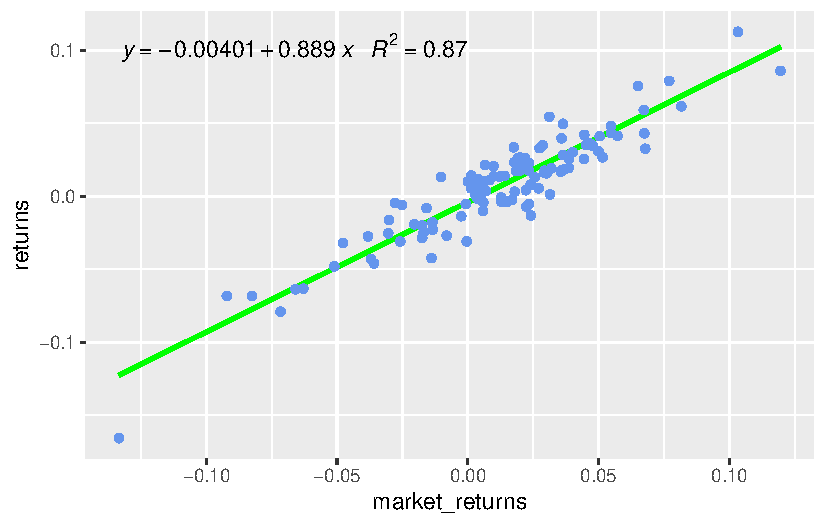
\includegraphics[width=0.4\linewidth,height=\textheight,keepaspectratio]{notebook_optimization_test_files/figure-pdf/unnamed-chunk-25-1.pdf}

\begin{center}\rule{0.5\linewidth}{0.5pt}\end{center}

\section{Tarea}\label{tarea}

\begin{enumerate}
\def\labelenumi{\arabic{enumi}.}
\item
  Calcule y analice la regresión entre los retorno del portafolio y los
  retornos del mercado. Genere conclusiones sobre la significancia y
  valores de los parámetros.
\item
  ¿Puede ser la pendiente de la regresión negativa?
\end{enumerate}




\end{document}
